\chapter{Requirements Analysis and Kanban Planning}

\section*{Introduction}
This chapter formalizes who uses Qatra, what the system must do, which qualities constrain the solution, and how work was organized as a continuous Kanban flow. The StarUML model supplied with the project is used as the principal use-case source and is cross-checked against controllers, services, frontend routes, and infrastructure files.

\section{System Actors}
The model identifies four human actors: donor, center staff, center administrator, and super administrator.

\begin{table}[H]
\centering\small
\begin{tabularx}{\textwidth}{|P{3.1cm}|Y|Y|}
\hline
\rowcolor{tableheader}\textbf{Actor} & \textbf{Main responsibilities} & \textbf{Data boundary}\\ \hline
Donor & Account, profile, health questionnaire, availability, centers, appointments, emergency responses & Own profile and authorized public/transactional data\\ \hline
Center staff & Schedule, check-in, eligibility review, screening, completion, no-show & Operational records for assigned center\\ \hline
Center administrator & Center registration, configuration, staff, slots, analytics, reports & Managed center and its staff/activity\\ \hline
Super administrator & Users, roles, center approval, GDPR, restrictions, global audit/reporting & Platform-wide governance data\\ \hline
System & Tokens, matching, notifications, eligibility, expiration, audit, forecasts & Service accounts and scheduled/event authority\\ \hline
\end{tabularx}
\caption{Qatra actors and authorization boundaries}
\label{tab:actors}
\end{table}

\section{Functional Requirements}

\diagram[0.57\textheight]{global-use-case}{Global Qatra use-case overview}

\subsection{Identity and Profile}
The system shall allow registration by email, email verification, login, logout, password reset, and controlled session management. A donor shall complete personal and health information, set blood type or mark it unknown, define notification preferences, and provide location manually or through GPS. Profile changes must be validated and subject to authorization.

\subsection{Donor Lifecycle}
A donor shall view and update availability, questionnaire answers, location, donation history, eligibility status, next eligible date, reliability score, impact information, and donation certificates. The system shall enforce cooldown rules after a completed donation and expose the result without asking the donor to infer medical dates.

\subsection{Centers and Appointments}
Users shall browse centers and view operating hours. Authorized administrators shall register and update centers, manage staff, configure slots, record operating-hour exceptions, and consult reports. Donors shall book, reschedule, cancel, and review appointments. Staff shall check in donors, record screening, complete appointments, and mark no-shows.

\subsection{Emergencies and Notifications}
Authorized users shall create, track, resolve, and review emergency requests. The system shall scan eligible donors, filter by compatibility and constraints, rank candidates, expand the radius when necessary, dispatch alerts, track delivery, and retry failed notifications. Donors shall view, accept, or decline requests.

\subsection{Administration and Governance}
Super administrators shall search users, change account status, approve or reject centers, assign or revoke roles, process deletion requests, review permanent health restrictions, consult dashboards, and export audit or platform reports. Every state-changing action should generate an attributable audit record.

\section{Non-Functional Requirements}
\begin{longtable}{|P{3.0cm}|P{7.1cm}|P{3.4cm}|}
\hline
\rowcolor{tableheader}\textbf{Quality} & \textbf{Requirement} & \textbf{Evidence or design response}\\ \hline
\endfirsthead
\hline\rowcolor{tableheader}\textbf{Quality} & \textbf{Requirement} & \textbf{Evidence or design response}\\ \hline
\endhead
Security & Authenticate API calls and authorize operations by role and resource scope & Spring Security, JWT dependencies, route guards, role-specific controllers\\ \hline
Privacy & Limit access to health, location, and deletion data & Role separation, GDPR use cases, audit model\\ \hline
Availability & Avoid coupling domain requests to slow notification channels & Kafka-oriented event exchange and separate notification service\\ \hline
Performance & Page list endpoints and avoid unnecessary frontend loading & Pagination utilities, feature routes, asynchronous processing\\ \hline
Consistency & Preserve appointment and slot constraints under concurrent requests & Transactional backend boundaries and explicit slot state\\ \hline
Maintainability & Keep domain rules separate from web and persistence details & Ports, adapters, domain models, DTOs, feature modules\\ \hline
Observability & Expose metrics, logs, and traces for distributed diagnosis & Actuator, Prometheus, Grafana, Loki, Promtail, Jaeger\\ \hline
Deployability & Package and update services reproducibly & Dockerfiles, Compose, k3s manifests, GitHub Actions\\ \hline
\caption{Principal non-functional requirements}
\label{tab:nfr}
\end{longtable}

\section{Product Backlog}
The backlog was organized by user value and dependency. Identity and foundational data precede appointments; appointments and health status precede reliable emergency matching; event exchange precedes real-time notification; operational visibility follows deployable services.

\begin{longtable}{|P{1.4cm}|P{3.6cm}|P{6.8cm}|P{2.0cm}|}
\hline
\rowcolor{tableheader}\textbf{ID} & \textbf{Epic} & \textbf{Representative outcome} & \textbf{Priority}\\ \hline
\endfirsthead
\hline\rowcolor{tableheader}\textbf{ID} & \textbf{Epic} & \textbf{Representative outcome} & \textbf{Priority}\\ \hline
\endhead
E1 & Identity and security & Verified account, login, reset, roles, protected routes & High\\ \hline
E2 & Donor onboarding & Health, blood type, location, availability, preferences & High\\ \hline
E3 & Center management & Center approval, staff, operating hours, slots & High\\ \hline
E4 & Appointment lifecycle & Booking, rescheduling, check-in, screening, completion & High\\ \hline
E5 & Donor engagement & History, eligibility, certificates, impact, reliability & Medium\\ \hline
E6 & Emergency management & Creation, deadline, progress, resolution, history & High\\ \hline
E7 & Matching engine & Compatibility, availability, distance, ranking, escalation & Medium\\ \hline
E8 & Notification engine & Alerts, retries, preferences, WebSocket updates & Low\\ \hline
E9 & Administration & Users, roles, restrictions, GDPR, audit & Medium\\ \hline
E10 & Analytics and reporting & Center and system summaries, exports & Low\\ \hline
E11 & Industrialization & CI/CD, containers, k3s deployment & Low\\ \hline
E12 & Observability & Metrics, dashboards, logs, traces & Low\\ \hline
\caption{Qatra product backlog by epic}
\label{tab:backlog}
\end{longtable}

\section{Kanban Method}
Kanban was selected because the work crossed analysis, backend, frontend, infrastructure, and documentation. A continuous pull system allowed an item to move when capacity existed rather than waiting for a sprint boundary~\cite{kanban}. Scrum instead organizes work through time-boxed Sprints, defined accountabilities, and recurring formal events~\cite{scrumGuide}. Table~\ref{tab:kanban-scrum} explains why Kanban was the more suitable project narrative. The working states were Backlog, Ready, In Progress, Review, Verification, and Done. Blocked work remained visible and did not count as completed.

\begin{table}[H]
\centering\small
\begin{tabularx}{\textwidth}{|P{3.0cm}|Y|Y|}
\hline
\rowcolor{tableheader}\textbf{Criterion} & \textbf{Scrum} & \textbf{Kanban and Qatra fit}\\ \hline
Delivery cadence & Work is planned and reviewed within fixed-length Sprints & Work can be pulled and completed continuously across backend, frontend, infrastructure, and report tasks\\ \hline
Change handling & Changes are normally considered without endangering the Sprint Goal & Priorities can be reordered whenever capacity becomes available\\ \hline
Flow control & Sprint Backlog and Sprint Goal guide the time box & Explicit work-in-progress limits expose overload and blocked work\\ \hline
Roles and events & Product Owner, Scrum Master, Developers, and prescribed events & No unsupported claim of historical Scrum roles or ceremonies is required\\ \hline
Project suitability & Strong when a stable team can sustain a regular Sprint rhythm & Better suited to an individual PFE with heterogeneous deliverables and variable task duration\\ \hline
\end{tabularx}
\caption{Kanban-versus-Scrum methodology justification}
\label{tab:kanban-scrum}
\end{table}

Work-in-progress limits protect focus. A reasonable individual-project policy is one principal implementation item and one review or documentation item in progress. This policy is described as the project method; no historical throughput figures are invented where no board export exists.

Figure~\ref{fig:kanban-reference} illustrates the visual pull principle adopted for the project. The detailed Qatra states remain Backlog, Ready, In Progress, Review, Verification, and Done.

\begin{figure}[H]
\centering
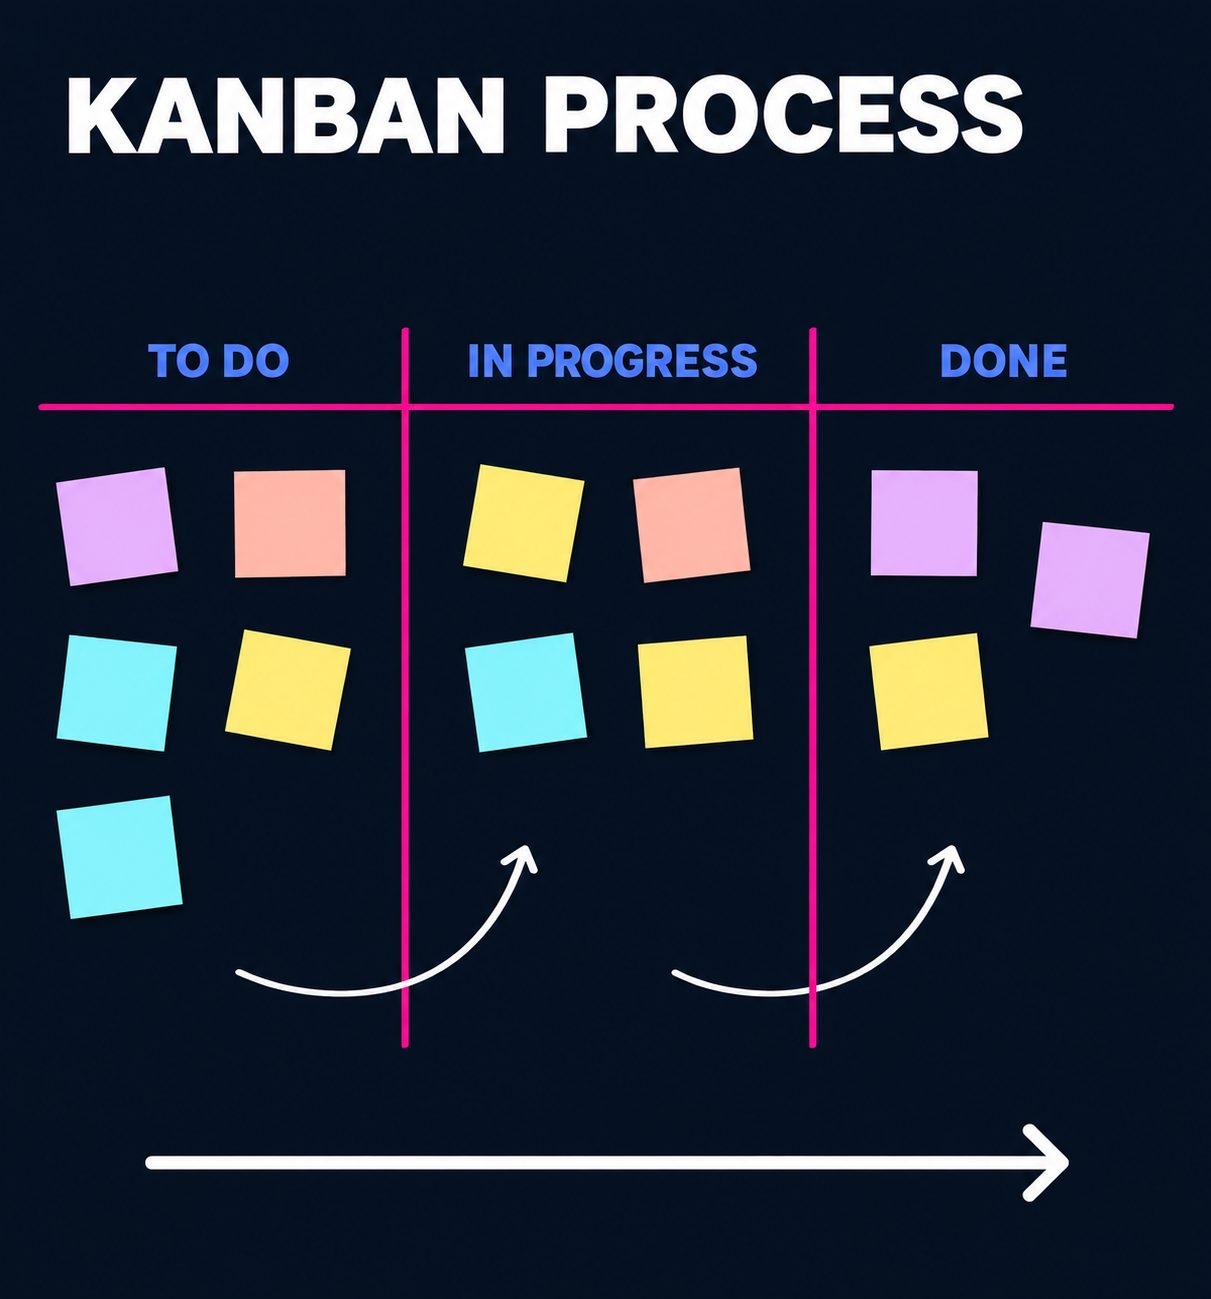
\includegraphics[height=0.34\textheight]{assets/methodology/Kanban-process.png}
\caption[Kanban process]{Kanban process}
\label{fig:kanban-reference}
\end{figure}

\section{Delivery Increments}
Kanban does not prevent grouping completed work into reportable increments. Six coherent increments are used for traceability:

\begin{enumerate}
  \item foundation, identity, and center management;
  \item donor profiles, center discovery, and appointments;
  \item staff operations and donation completion;
  \item emergency request lifecycle;
  \item matching, notifications, and real-time updates;
  \item analytics, administration, deployment, and observability.
\end{enumerate}

\diagram[0.25\textheight]{increment-roadmap}{Functional dependency roadmap for Kanban increments}

\section{Definition of Done and Traceability}
A work item is considered done when its acceptance behavior is implemented, authorization and validation have been considered, affected interfaces are documented, and available automated checks pass in the intended CI environment. Where verification cannot be reproduced locally, the limitation is recorded instead of replacing evidence with an assumption.

Traceability is maintained from actor needs to backlog epics, domain modules, frontend features, tests, and diagrams. Table~\ref{tab:traceability} gives representative examples.

\begin{table}[H]
\centering\small
\begin{tabularx}{\textwidth}{|P{3.2cm}|P{3.0cm}|Y|Y|}
\hline
\rowcolor{tableheader}\textbf{Need} & \textbf{Epic} & \textbf{Backend evidence} & \textbf{Frontend evidence}\\ \hline
Book a donation slot & E4 & Appointment application/domain/web modules & Slot booking page and appointment models\\ \hline
Operate a center & E3/E4 & Center and appointment modules & Center management and staff pages\\ \hline
Respond to an emergency & E6/E7 & Emergency and matching responsibilities & Emergency list/detail pages\\ \hline
Receive timely updates & E8 & Notification service and event configuration & Notification service, store, bell, and center page\\ \hline
Audit administrative actions & E9 & Analytics audit log module & Staff activity and administrative views\\ \hline
\end{tabularx}
\caption{Representative requirement-to-implementation traceability}
\label{tab:traceability}
\end{table}

\section*{Conclusion}
The requirements and backlog establish a controlled functional scope, while Kanban explains how value was delivered continuously. The next chapter shows how these requirements are mapped to services, modules, data stores, security controls, and deployment nodes.
